\documentclass[tikz,border=2pt]{standalone}
\usepackage{amsmath,amssymb}
\usepackage{tikz}

\begin{document}
% Sequentially compact: every sequence in E has a subsequence converging to a point of E.
% In the closed disc the highlighted subsequence settles at a limit inside E; in the open disc
% a sequence can creep to the rim, whose points are missing.
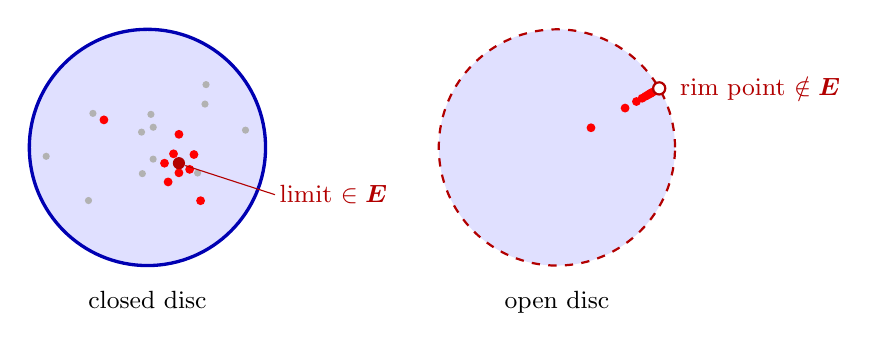
\begin{tikzpicture}[every node/.style={font=\small}]
	\fill[blue!12] (0,0) circle (1.5);
	\draw[blue!70!black, very thick] (0,0) circle (1.5);
	\foreach \i in {1,...,12} {
		\pgfmathsetmacro{\r}{1.3*(0.55+0.45*cos(70*\i))}
		\pgfmathsetmacro{\a}{37*\i}
		\fill[gray!60] ({\r*cos(\a)},{\r*sin(\a)}) circle (1.3pt);
	}
	\foreach \i in {1,...,9} {
		\pgfmathsetmacro{\r}{1.1/\i}
		\pgfmathsetmacro{\a}{150*\i}
		\fill[red] ({0.4+\r*cos(\a)},{-0.2+\r*sin(\a)}) circle (1.6pt);
	}
	\fill[red!70!black] (0.4,-0.2) circle (2.2pt);
	\draw[red!70!black, thin] (0.48,-0.23) -- (1.62,-0.6);
	\node[red!70!black, anchor=west, inner sep=1.5pt] at (1.62,-0.6) {limit $\in\boldsymbol{E}$};
	\node[anchor=north] at (0,-1.7) {closed disc};
	\begin{scope}[xshift=5.2cm]
		\fill[blue!12] (0,0) circle (1.5);
		\draw[red!70!black, thick, dashed] (0,0) circle (1.5);
		\foreach \i in {1,...,10} {
			\pgfmathsetmacro{\r}{1.5-1.0/\i}
			\fill[red] ({\r*cos(30)},{\r*sin(30)}) circle (1.6pt);
		}
		\draw[red!70!black, thick, fill=white] ({1.5*cos(30)},{1.5*sin(30)}) circle (2.2pt);
		\node[red!70!black, anchor=west] at ({1.55*cos(30)+0.1},{1.5*sin(30)}) {rim point $\notin\boldsymbol{E}$};
		\node[anchor=north] at (0,-1.7) {open disc};
	\end{scope}
\end{tikzpicture}
\end{document}
